\documentclass[a4paper,10pt]{article}

\usepackage{graphicx}
\graphicspath{{sections/images/}}

\usepackage{amsmath}
\usepackage{amsfonts}
\usepackage{amssymb}
\usepackage{hyperref}
\usepackage[a4paper, top=2cm, bottom=2cm, left=2.5cm, right=2.5cm]{geometry}
\usepackage{caption}
\usepackage{graphicx}

\begin{document}
\begin{titlepage}
    \centering  
    \begin{figure}[ht]
        \centering
        
\includegraphics[width=\textwidth]{ise-logo.png}
    \end{figure}
    \vspace*{2cm} 
    
    {\Huge Progress Report 2\par}
    \vspace{1cm}
    
    {\Huge \textit{Pookie: An AI-Driven Robot for Promoting Mental Wellbeing and Emotional Support} \par}
    \vspace{3cm}
    
    {\large \textbf{Authors:} Tibet Buramarn, Kridbhume Chammanard, and Thitaya Divari \par}
    \vspace{1cm}
    {\large \textbf{Advisor:} Dr. Paulo Fernando Rocha Garcia and \par}
    {\large Ms. Kunpariya Siripanit \par}

    \vspace{3cm}
    
    {\large 2147416 Final Project I \par}
    {\large International School of Engineering (ISE) \par}
    {\large Chulalongkorn University \par}
    
    \vspace{2cm}
    
    {\large October 25, 2024 \par}
    
    \vspace*{\fill}
\end{titlepage}

\thispagestyle{empty}

\newpage
\tableofcontents

\newpage
\section{Introduction}
This progress report provides an update on the development of Pookie, an AI-driven robot designed to promote mental well-being, developed in assistance from Chula Student Wellness. Pookie aims to act as a companion to help alleviate feelings of stress and anxiety, especially in response to future societal concerns like "Terror Outbursts," an anxiety-driven phenomenon anticipated to affect Thailand. The project focuses on enhancing positivity and emotional attachment by creating a robot that interacts with users in an empathetic and calming manner.

\section{Overview}
As a quick recap for how Pookie works, the robot utilizes video and audio sensors to predict the user’s current facial and speech emotion. This is done through using convolutional neural networks for facial emotion recognition, and bidirectional LSTMs for speech emotion recognition. The robot processes the user’s inputs and determines the best interaction for the user. For instance, if the user seems to be down or sad, Pookie might choose to make a soft and calming sound, a cheerful face, and slow movements in order to emotionally engage with the user, supposedly attempting to empathize with the user. With that said, this section will provide an overview into Pookie’s implementation in semester 2, detailing what’s done, what’s being doing, and what needs to be done next.
\subsection{What’s done}
Overall, the team has finalized the overarching approach of the interaction with the robot. This process was not well defined in the last semester, which led to ambiguity towards the final presentation. To elaborate, it was not clear of what output the robot would elicit given a certain combination of emotions. If the user was sad, should the robot try to cheer the user up? Or should it maintain neutrality. As such, the team has decided to consult Chula Student Wellness again for a quick chat to obtain their thoughts on this problem. They told us that the factors going into determining the output were almost infinite, where even psychologists themselves have problems truly empathizing with a person, and determining what to do to make a person feel better. As such, they claim it is almost impossible for our project to empathize to that extent. Therefore, we settled on a more generalized approach, as shown in Figure \ref{fig:flow}.

\begin{figure}[ht]
    \centering
    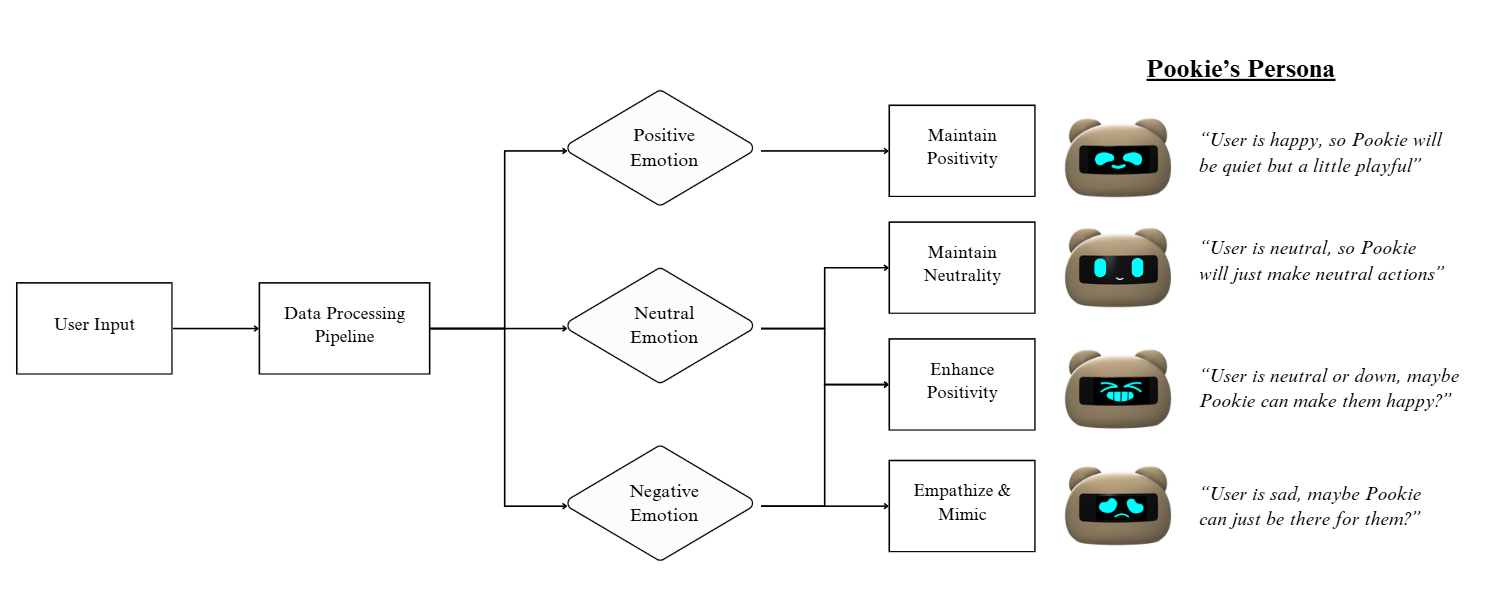
\includegraphics[width=\textwidth]{flow.png}
    \caption{Pookie Interaction Flowchart}
    \label{fig:flow}
\end{figure}

After processing inputs in the form of facial and speech emotion, the robot segments the output into 3 possible cases: positive, neutral and negative. With each case, the robot has a set of outputs it can perform. For instance, if the person is in a positive wellness state, Pookie will maintain positivity, meaning its intention will be to ensure this positive state of being of the user will be prolonged. On the other hand, if the user is neutral, Pookie will try to maintain this neutrality, but in some cases, such as if our models detect that the user is 60\% neutral, but 40\% happy, then the robot will elicit an output that could potentially make the user happier. Lastly, for the case of negative emotion, this part is tricky. The team has a design problem here: if the user is feeling negative, should the robot remain neutral? Should it show empathy? Or should it be fun and energetic? The underlying emotional factors, as we mentioned, are almost infinite, so we simplified it into two cases: either enhance positivity or empathize. In the case of empathy, the robot will simply mimic the user’s emotion (e.g sadness), with the intention of “being there” for the user. 

Another fundamental update is how Pookie processes the emotional inputs. Initially, the team finalized on the approach of finding the dominant emotion from the facial and speech emotion recognition models within a given time frame, then simply using those two dominant emotions to elicit an input. For instance, within 10 seconds, if a user made a “happy” face, and their speech is “happy”, then the output would be a positive maintenance. However, this approach disregarded many cases and made the robot very static. If the user’s face is “sad”, but their voice is “happy”, it’s impossible to combine these emotions and determine what the user’s true emotion is. This leads us to incorporating two new key technologies: bayesian networks and decision trees, creating a new flowchart as seen in Figure \ref{fig:rev_flow}.

\begin{figure}[ht]
    \centering
    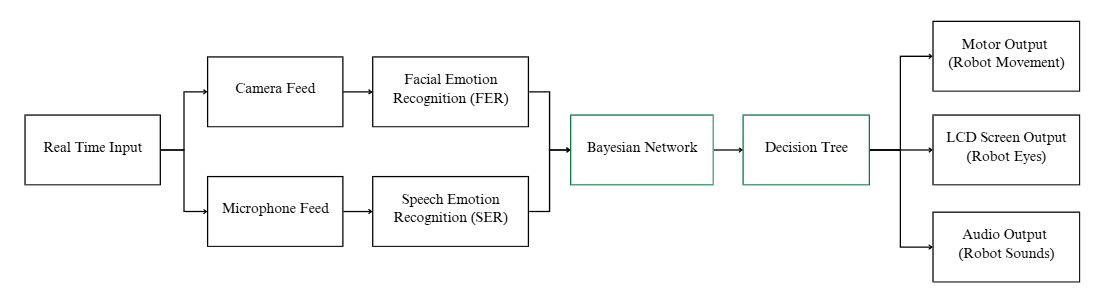
\includegraphics[width=\textwidth]{flow_revised.png}
    \caption{Revised Flowchart for Input Processing}
    \label{fig:rev_flow}
\end{figure}

The next update involves the implementation of the robot’s eyes, which is a fundamental interaction done through the LCD screen of the robot. Initially, the eyes of the robot used a Python library called OpenCV, which is an image processing library allowing the drawing of various shapes. The eyes were hard coded as various shapes and patterns drawn on a black canvas, as shown in Figure 3. The main challenge with this approach was the scalability and implementation time. Since each frame is hard coded, it does not allow for much flexibility and complex shapes. However, the upside is that it can easily be built in as a class into the main code. 

\begin{figure}[ht]
    \centering
    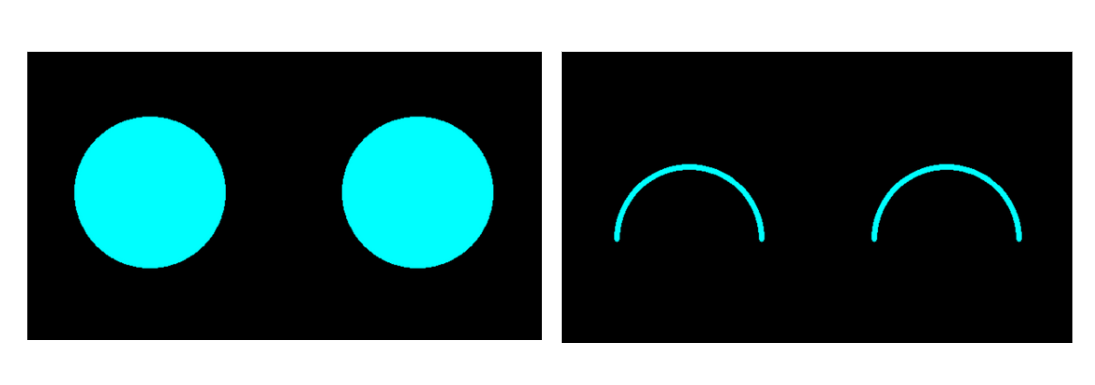
\includegraphics[width=\textwidth]{happy.png}
    \caption{OpenCV Eyes Example for “Happy”}
    \label{fig:happy}
\end{figure}

The team decided on a different approach: using a simple software that could easily create dynamic shapes and record the frame sequence as a common file type, like GIF. The solution was Canva, a program typically used to make powerpoint slides, but with animation capabilities as well. Through implementing the eye sequence as a GIF format instead of hard coding, we are able to achieve more unique and personalized eye shapes and sequences for Pookie. Some examples of these are shown in Figure \ref{fig:new_eyes}.

\begin{figure}[ht]
    \centering
    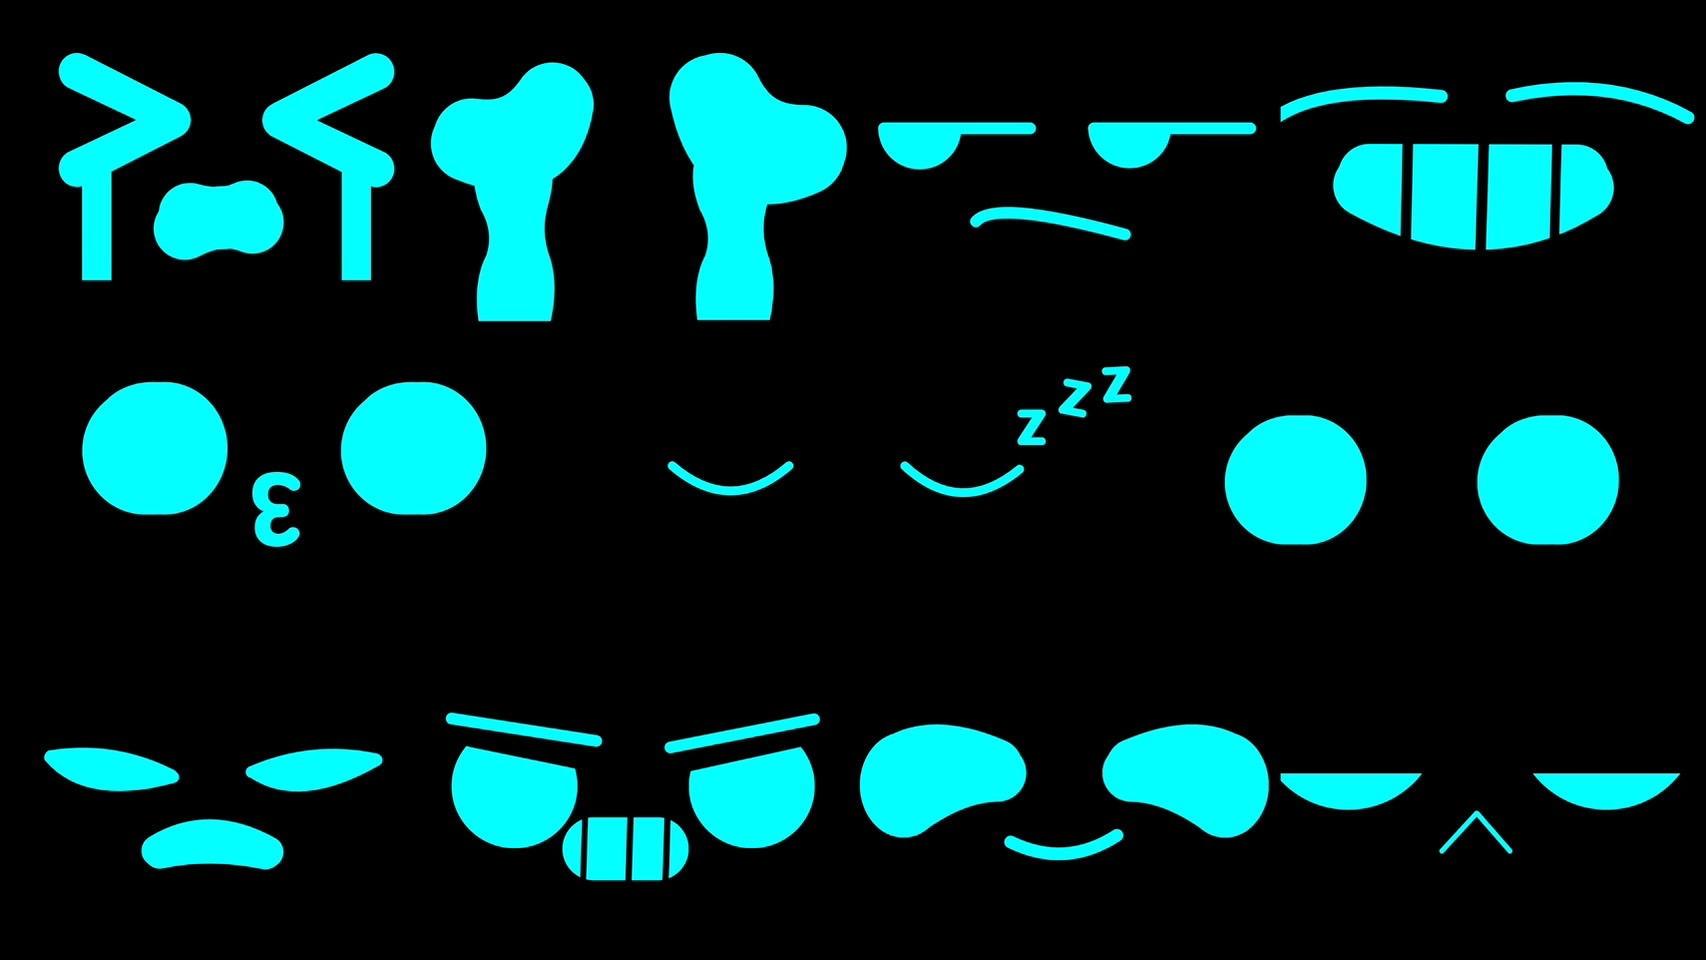
\includegraphics[width=\textwidth]{new_eyes.png}
    \caption{New Eyes Drawn as GIF Sequence on Canva}
    \label{fig:new_eyes}
\end{figure}

\newpage
Lastly, some other updates regard the hardware components. Our hardware team has completed a final design of Pookie in Fusion 360, and has acquired almost all necessary components needed for assembly. This will be discussed further in the hardware section.

\subsection{What we are working on}
This section discusses the currently ongoing tasks the team is working on this week and next week. Currently, the team is working on the Jetson Nano integration, which is the main processor for the project. Initially, in the last semester, the code, sensors, models, and so on were all hosted on a local computer, so it must be migrated and tuned so that it works appropriately with the Jetson Nano. Aside from this, we are working on coding the hardware functions, such as driving the servo motors, which are used to drive the arms, base, and neck of the robot. 

On the software side, although we have completed the Bayesian network, which is essential for predicting the user’s true emotion, the next part is also challenging: the decision tree. This requires the team to carefully design and process inputs. For instance, if the user is detected to be 50\% happy and 50\% sad at the same time, what does this constitute? Which set of actions should the robot perform: positive enhancement or maintenance. The team is working on carefully building this tree everyday, a few nodes at a time.


\newpage
\section{Facial Expression Recognition}
The development of the Pookie AI-driven robot incorporates a crucial element: detecting and interpreting user emotions, particularly stress and anxiety, using Facial Emotion Recognition (FER). This section outlines the current progress, challenges, and future approaches for designing the emotion detection system, including relevant datasets, models, and methodologies.
\subsection{As-is Behavior}
Initially, the facial expression recognition model for this project was expected to use a model fine tuning approach over a Chinese Faces Dataset, as it provides the most symmetric resemblance to a Thai dataset, which is difficult to obtain. The foundation model used was a VGGNet architecture (Figure 2), a multi layer convolutional neural network often used for feature extraction and classification tasks, with a notable variety of emotion detection models stemming from it. 

\begin{figure}[ht]
    \centering
    \captionsetup{justification=centering}
    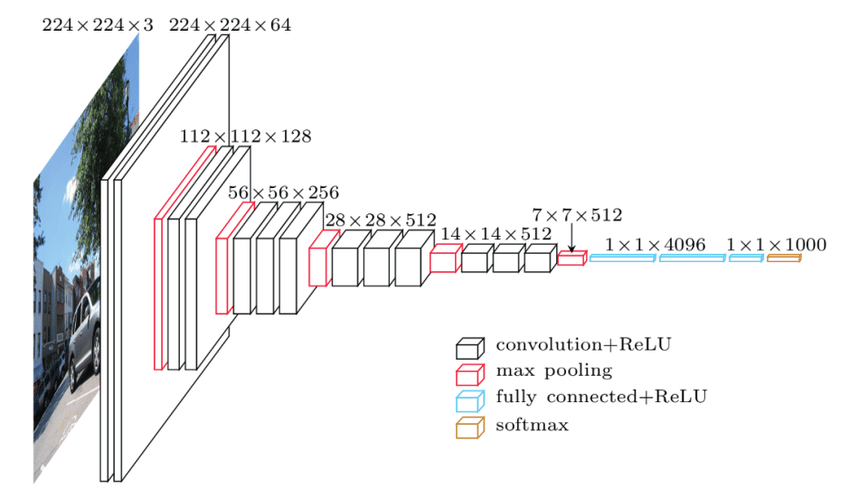
\includegraphics[width=0.9\textwidth]{vggnet.png}
    \caption{VGGNet Architecture}
    \label{fig:vggnet}
\end{figure}

For our approach, we took a pre-trained model for emotion recognition using VGGNet architecture, then fine tuned the inference layers on a Chinese dataset in order to get more accurate representation for Thai faces. The other layers were frozen, and served as foundation parameters for transfer learning. After multiple versions of the model, however, it could be seen that this approach did not yield great results. As shown in Figure 3, the model yielded results far worse than simple guessing, most likely due to inappropriate usage of transfer learning on an already imperfect model. 

\begin{figure}[ht]
    \centering
    \captionsetup{justification=centering}
    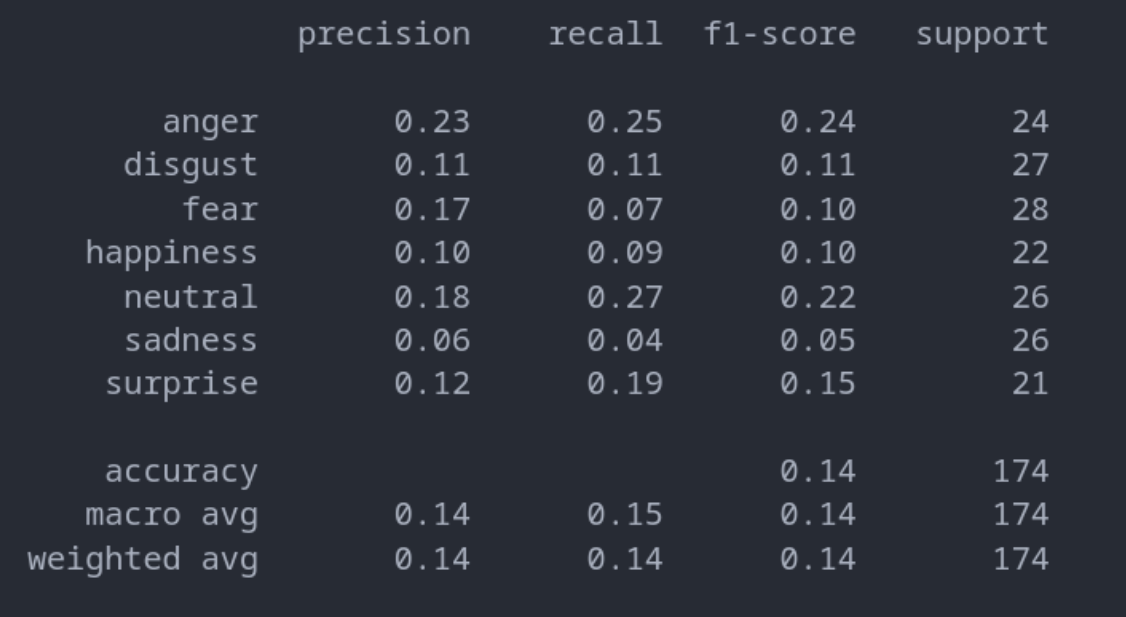
\includegraphics[width=0.67\textwidth]{finetune.png}
    \caption{Fine Tuning Results}
    \label{fig:finetune}
\end{figure}

\newpage
\subsection{Refined Approach}
After consultation with our advisor, we were recommended to revise our research on facial emotion recognition, where some of the assumptions and approaches we had initially proven to be wrong. Initially, the fine tuning approach was meant to familiarize the pre-trained VGGNet with a new dataset that could be ignored or underrepresented. However, the use case of fine tuning and transfer learning requires careful consideration. Thus, instead of fine tuning the model over the Chinese dataset, we instead included the Chinese dataset in the training and validation sets, where instead of using pre-trained weights, we trained an emotion detection model following the VGGNet architecture from scratch, which yielded significantly better results, as shown in Figure 4.

\begin{figure}[ht]
    \centering
    \captionsetup{justification=centering}
    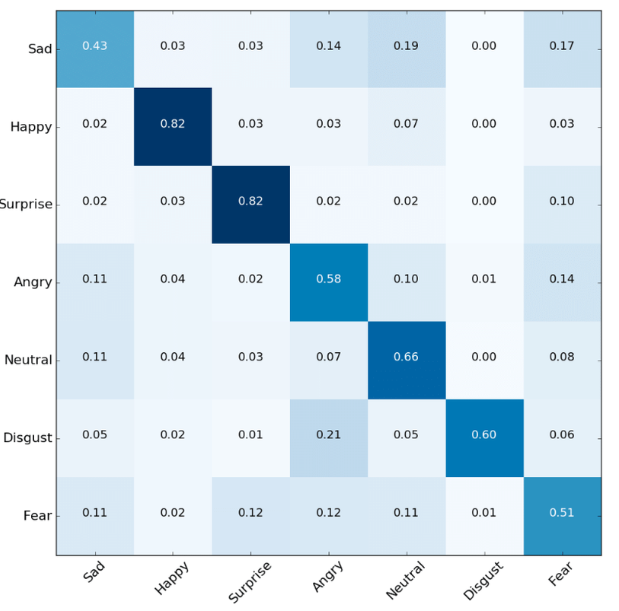
\includegraphics[width=0.8\textwidth]{refined.png}
    \caption{Refined Approach Results}
    \label{fig:refined}
\end{figure}

As seen in the results, the model is great at distinguishing between positive emotions such as happiness or surprise, but it is quite lacking in negative emotions. However, given the scope of the project, where positive and neutral are associated with specific outputs, and negative emotions are all classified as stress, then the model is generally enough to use as a minimum viable product for the rest of the semester.

\subsection{Next Steps}
The next steps for facial emotion recognition is to integrate this model with the SER server to have a common ground for communication and output. Although the model is not perfect, it is viable enough to be used for a prototype for the rest of the semester, where other parts will be prioritized from now on.

\newpage
\section{Speech Emotion Recognition}
Another key element of Pookie’s AI is the Speech Emotion Recognition (SER) system, which is used for recognizing the user’s emotions based on vocal patterns. By analyzing factors such as pitch, tone, and intensity, the system detects emotions: neutral, anger, happiness, sadness, and frustration. This section outlines the current progress, challenges, and future approaches for designing the speech emotion recognition model, including relevant datasets and methodologies.
\subsection{Speech Emotion Recognition Model}
We are utilizing a dataset created by Chulalongkorn University in collaboration with VISTEC, DEPA, and AIS, containing 41 hours and 36 minutes of audio recordings labeled with five emotions: neutral, anger, happiness, sadness, and frustration. VISTEC has also developed a speech emotion recognition model based on this dataset. We are in the process of adjusting the model's parameters to better fit our system.

\subsubsection*{Parameters:}

\begin{itemize}
    \item \textbf{Number of Mel-filterbanks:} Mel-filterbanks are used to transform the frequency spectrum into a scale that better aligns with how humans perceive sound. By adjusting the number of filterbanks, we can control the resolution of this transformation, which affects the granularity of frequency representation in the model. More filter banks provide finer detail, while fewer filterbanks reduce the model’s sensitivity to frequency variations.
    \item \textbf{Sampling Rate:} The sampling rate refers to how many samples per second the audio is recorded or processed. A higher sampling rate captures more detail from the audio signal, but it also increases the computational load. Adjusting this parameter ensures that the audio quality is sufficient for emotion recognition without overwhelming system resources.
    \item \textbf{Frame Length of STFT:} The STFT converts audio signals into a time-frequency representation. The frame length defines how long each segment of audio is for this transformation. A longer frame provides more frequency resolution but less time precision, while a shorter frame offers better time resolution but less frequency detail. Balancing these is key for accurate emotion recognition.
    \item \textbf{Epochs:} This parameter refers to the number of times the entire training dataset passes through the model during training. Adjusting the number of epochs affects how well the model learns from the data. Too few epochs may lead to underfitting, where the model doesn’t learn enough, while too many can cause overfitting, where the model memorizes the training data but performs poorly on new data.

\end{itemize}

The results are as shown in Figure 3, Figure 4, and Figure 5.

\begin{figure}[ht]
    \centering
    \captionsetup{justification=centering}
    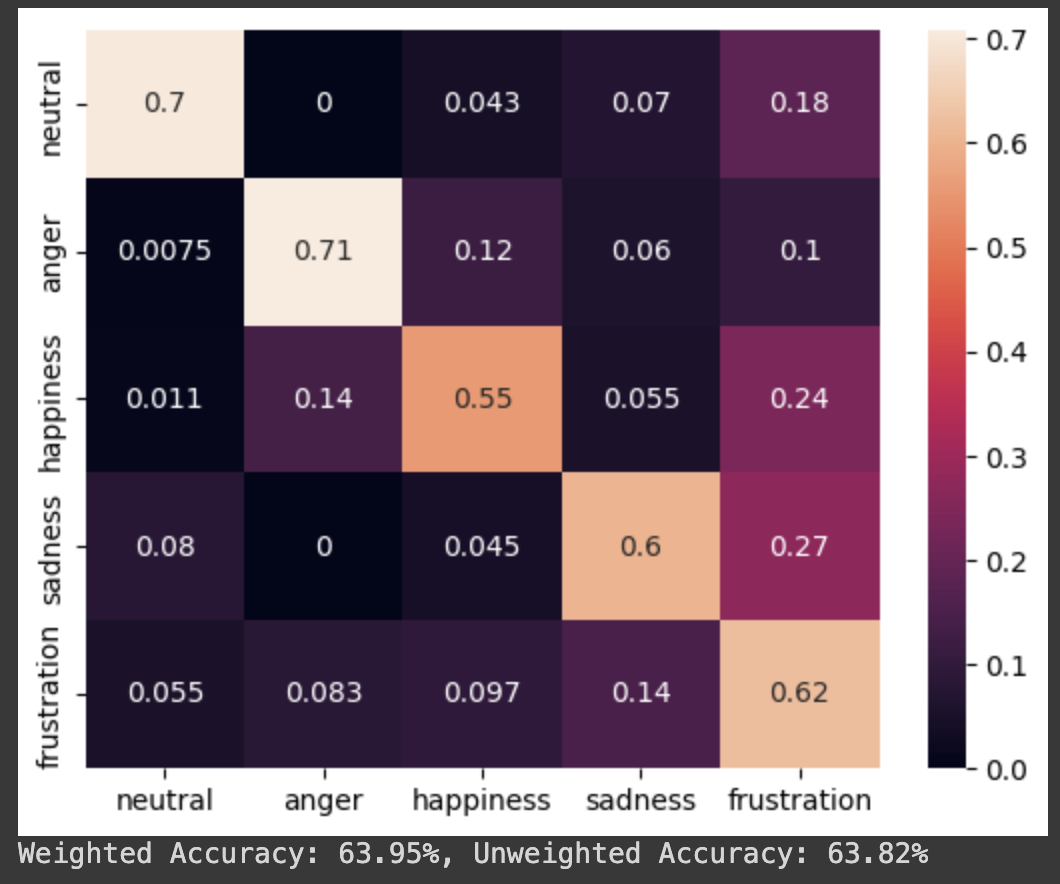
\includegraphics[width=0.5\textwidth]{default.png}
    \caption{Default parameters with 80 mel-filterbanks, sampling rate at 16,000 Hertz, and frame length of STFT at 50 milliseconds at 80 epochs}
    \label{fig:default}
\end{figure}

\begin{figure}[ht]
    \centering
    \captionsetup{justification=centering}
    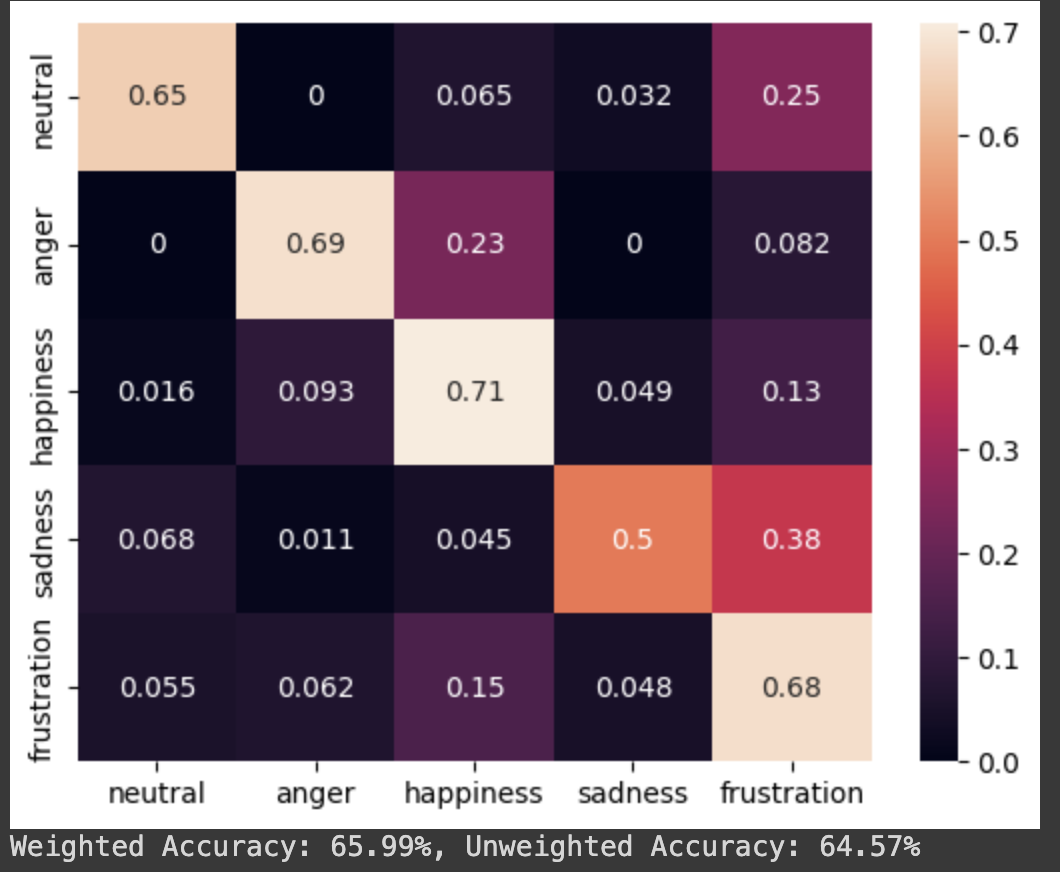
\includegraphics[width=0.5\textwidth]{128m-22050.png}
    \caption{Tuned model with 128 mel-filterbanks, sampling rate at 22,050 Hertz, and frame length of STFT at 50 milliseconds at 60 epochs}
    \label{fig:128m-22050}
\end{figure}

\begin{figure}[ht]
    \centering
    \captionsetup{justification=centering}
    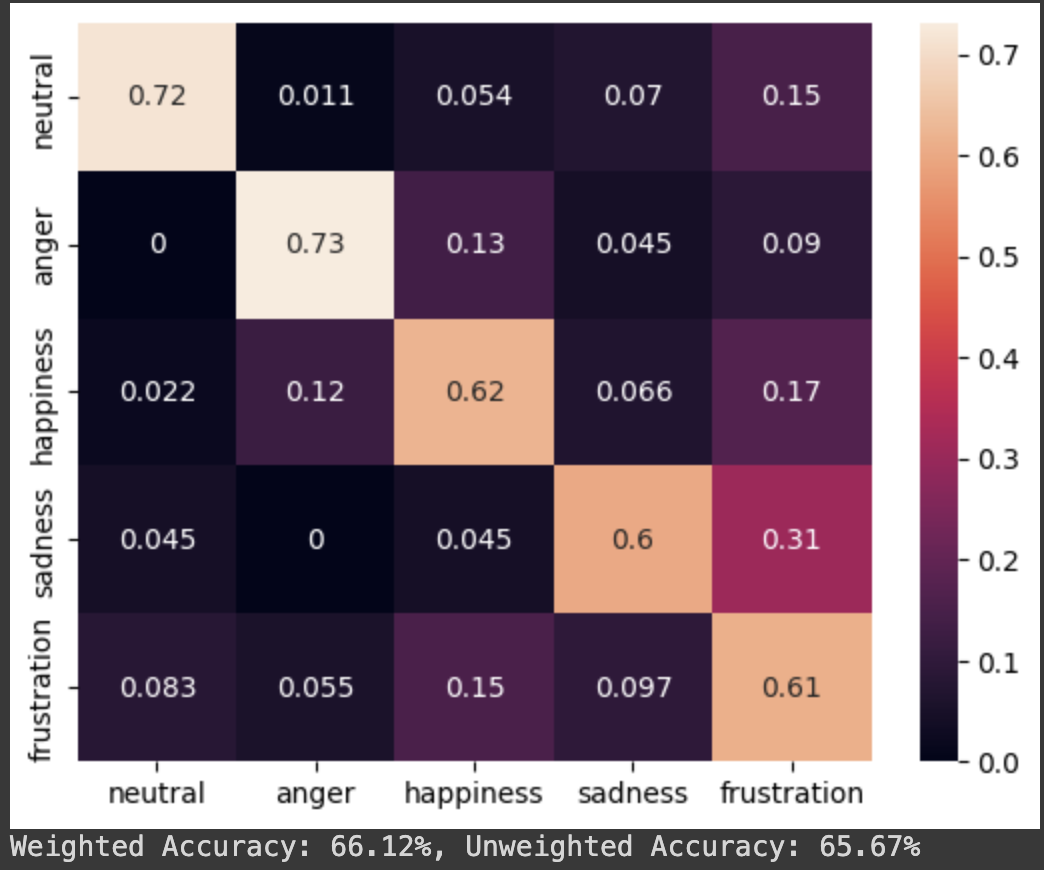
\includegraphics[width=0.5\textwidth]{128m-25ms.png}
    \caption{Tuned model with 128 mel-filterbanks, sampling rate at 16,000 Hertz, and frame length of STFT at 25 milliseconds at 60 epochs}
    \label{fig:128m-25ms}
\end{figure}

\subsection{Design Challenges}
Similarly to the FER, the input-output interaction for SER also poses a significant challenge:
\begin{itemize}
    \item \textbf{Defining input/output structure:} This design challenge which was addressed for FER is also present in SER as these two systems are intertwined and SER’s initialization might depend on other factors such as duration of facial detection. As of the report this is still under discussion as mentioned in the FER section.
\end{itemize}
    
    Overall, the current design issues of the SER stems from undecided input and output structure and interactions, both of which will be addressed by the next progress report in October.

\subsection{Technical Challenges}
Several technical challenges have emerged, primarily related to compatibility:
\begin{itemize}
    \item \textbf{Compatibility issues:} The original SER model was created three years ago, and since then, Google Colab has updated its Python version from 3.7 to 3.10, alongside a CUDA update to version 12.1. Python 3.7 reached its end of life (EOL) as of June 27, 2023, which has caused compatibility issues with the model's required libraries. The mismatch between Google Colab’s Python environment and the model’s requirements has led to several errors. To address this, we created a forked version of the original VISTEC-SER model and modified it according to the updated dependencies which include a plethora of changes to the source code.
\end{itemize}
\section{Robot Design}
\subsection{Fusion360 CAD Implementation}
Significant progress has been achieved in the hardware development phase of the Pookie robot. The outer shell design, now at 80\% completion, has been crafted using Fusion360 CAD software, ensuring precise dimensional accuracy and manufacturability. This development phase has focused on creating a structurally sound and aesthetically cohesive external framework.

\begin{figure}[ht]
    \centering
    \captionsetup{justification=centering}
    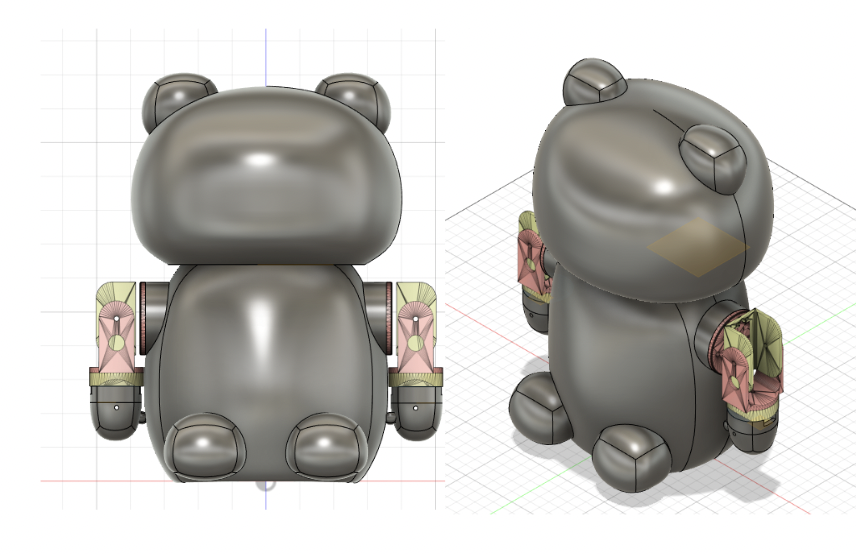
\includegraphics[width=\textwidth]{cad.png}
    \caption{Pookie CAD Implementation}
    \label{fig:cad}
\end{figure}

The robotic arm mechanism represents a completed milestone in the project's development cycle. Through comprehensive mechanical analysis and iterative design refinement, the arm assembly has been successfully engineered to meet all operational requirements. The integration of DS3255 servo motors has been a crucial element in this design phase, with their specifications carefully incorporated to ensure optimal torque delivery and precise movement control.

\begin{figure}[ht]
    \centering
    \captionsetup{justification=centering}
    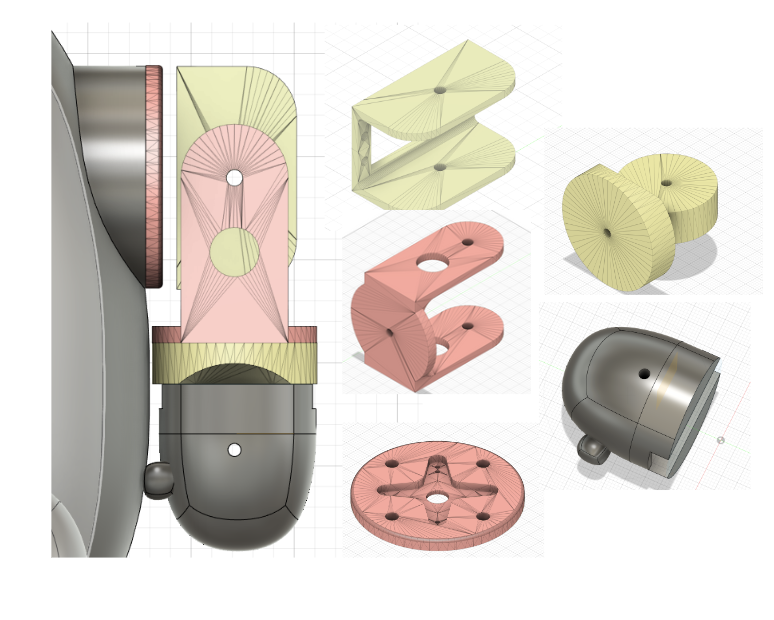
\includegraphics[width=0.7\textwidth]{arm.png}
    \caption{Pookie Robotics Arm Mechanism}
    \label{fig:arm}
\end{figure}

\newpage
The inner shell architecture remains under active development, with significant progress made on critical mechanical components. The servo motor housing for the DS3255 units has been successfully designed in Fusion360, ensuring precise mounting and optimal operational performance. However, the upper head assembly is still in the design phase, requiring further refinement. Concurrent development is underway for the integration frameworks of essential components, including sensor mounting brackets, speaker housings, and LED eye assemblies. This systematic approach to the inner architecture ensures proper component placement while maintaining the structural integrity of the design.

\begin{figure}[ht]
    \centering
    \captionsetup{justification=centering}
    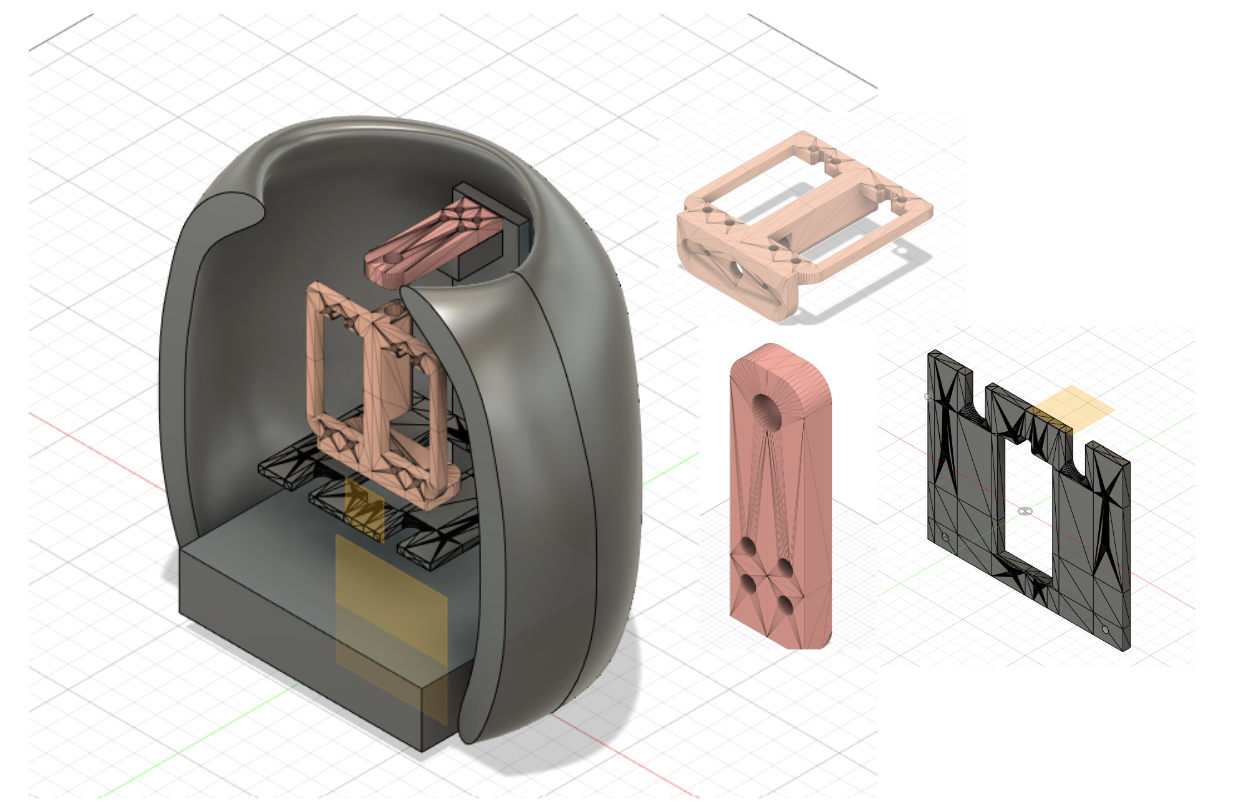
\includegraphics[width=0.7\textwidth]{inner.png}
    \caption{Pookie Inner Shell Design}
    \label{fig:inner}
\end{figure}


\end{document}
